\documentclass[tikz]{standalone}

\usepackage{xstring}

\usetikzlibrary{fit,positioning}

\newcommand\drawNodes[2]{
  % #1 (str): namespace
  % #2 (list[list[str]]): list of labels to print in the node of each neuron
  \foreach \neurons [count=\lyrIdx] in #2 {
    \StrCount{\neurons}{,}[\layerLen] % use xstring package to save each layer size into \layerLen macro
    \foreach \n [count=\nIdx] in \neurons
      \node[neuron] (#1-\lyrIdx-\nIdx) at (2*\lyrIdx, \layerLen/2-1.4*\nIdx) {\n};
  }
}

\newcommand\denselyConnectNodes[2]{
  % #1 (str): namespace
  % #2 (list[int]): number of nodes in each layer
  \foreach \n [count=\lyrIdx, remember=\lyrIdx as \previdx, remember=\n as \prevn] in #2 {
    \foreach \y in {1,...,\n} {
      \ifnum \lyrIdx > 1
        \foreach \x in {1,...,\prevn}
          \draw[->] (#1-\previdx-\x) -- (#1-\lyrIdx-\y);
      \fi
    }
  }
}

\begin{document}
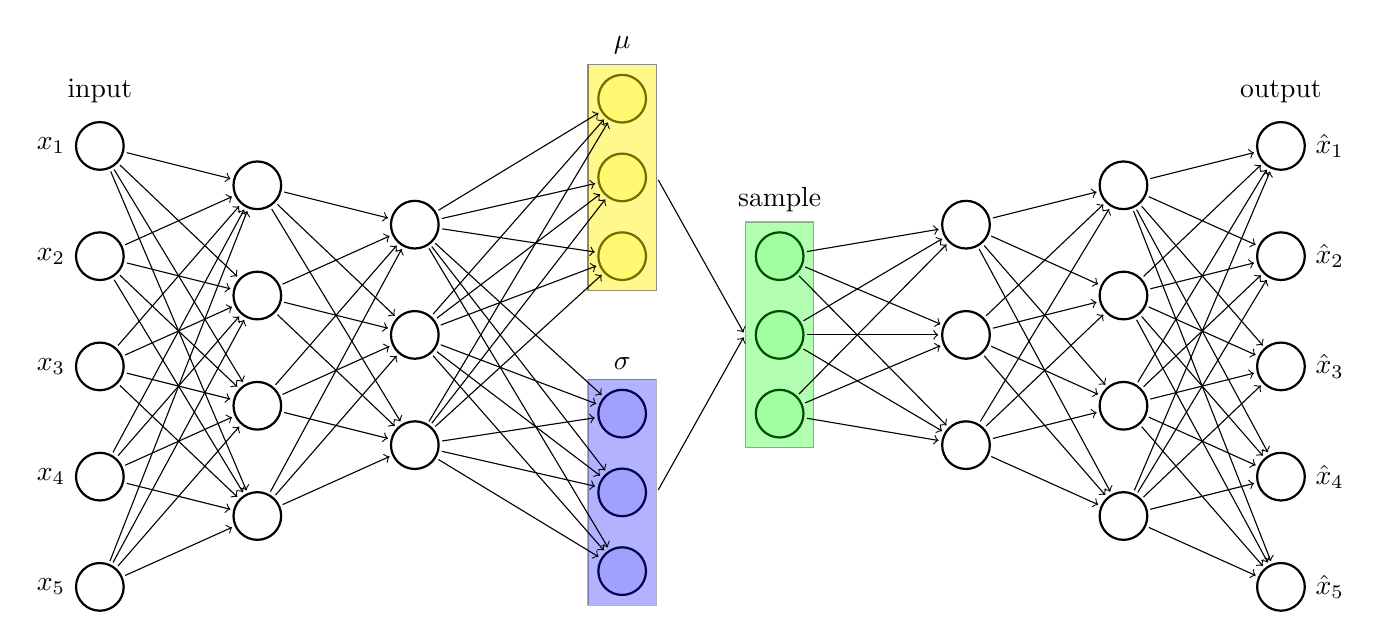
\begin{tikzpicture}[
    shorten >=1pt, shorten <=1pt,
    neuron/.style={circle, draw, minimum size=4ex, thick},
    legend/.style={font=\large\bfseries},
  ]

  % encoder
  \drawNodes{encoder}{{{,,,,}, {,,,}, {,,}}}
  \denselyConnectNodes{encoder}{{5, 4, 3}}

  % decoder
  \begin{scope}[xshift=11cm]
    \drawNodes{decoder}{{{,,}, {,,,}, {,,,,}}}
    \denselyConnectNodes{decoder}{{3, 4, 5}}
  \end{scope}

  % mu, sigma, sample nodes
  \foreach \idx in {1,...,3} {
      \coordinate[neuron, right=2 of encoder-3-2, yshift=\idx cm,, fill=yellow, fill opacity=0.2] (mu-\idx);
      \coordinate[neuron, right=2 of encoder-3-2, yshift=-\idx cm, fill=blue, fill opacity=0.1] (sigma-\idx);
      \coordinate[neuron, right=4 of encoder-3-2, yshift=\idx cm-2cm, fill=green, fill opacity=0.1] (sample-\idx);
    }

  % mu, sigma, sample boxes
  \node [label=$\mu$, fit=(mu-1) (mu-3), draw, fill=yellow, opacity=0.45] (mu) {};
  \node [label=$\sigma$, fit=(sigma-1) (sigma-3), draw, fill=blue, opacity=0.3] (sigma) {};
  \node [label=sample, fit=(sample-1) (sample-3), draw, fill=green, opacity=0.3] (sample) {};

  % mu, sigma, sample connections
  \draw[->] (mu.east) edge (sample.west) (sigma.east) -- (sample.west);
  \foreach \a in {1,2,3}
  \foreach \b in {1,2,3} {
      \draw[->] (encoder-3-\a) -- (mu-\b);
      \draw[->] (encoder-3-\a) -- (sigma-\b);
      \draw[->] (sample-\a) -- (decoder-1-\b);
    }

  % input + output labels
  \foreach \idx in {1,...,5} {
      \node[left=0 of encoder-1-\idx] {$x_\idx$};
      \node[right=0 of decoder-3-\idx] {$\hat x_\idx$};
    }
  \node[above=0.1 of encoder-1-1] {input};
  \node[above=0.1 of decoder-3-1] {output};

\end{tikzpicture}
\end{document}
